We evaluate our planned protest detection system
using metrics similar to those described by Ramakrishnan et al.~\cite{emberskdd} in evaluating their work.
Given a set of alerts issued by the system and the GSR comprising actual protest incidents, we aim to identify
a correspondence between the two sets via a bipartite matching.
An alert can be matched to a GSR event only if i) they are both issued for the same country, 
ii) the alert's predicted location and the event's reported location are within 300km of each
other (the distance offset), and iii) the forecasted event date is within a given interval of the true event date (the date offset).
Once these inclusion criteria apply, the quality score (QS) of the match is defined as a combination of the
location score (LS) and date score (DS):
\begin{equation}
    \operatorname{QS}= (LS + DS)*2
\end{equation}
\noindent
where
\narenc{equations are wrong! Need a scaling factor if LS and DS are supposed to lie in [0,1].}
\begin{equation}
    \operatorname{LS}=1 - \frac{\min(\textrm{distance offset}, 300)}{300}
\end{equation}
and 
\begin{equation}
    \operatorname{DS}=1 - \frac{\min(\textrm{date offset}, \operatorname{INTERVAL})}{\operatorname{INTERVAL}}
\end{equation}
Here, we explore $\operatorname{INTERVAL}$ values from $0$ to $7$.
if an alert (conversely, GSR event) cannot be matched to any GSR event (alert, respectively), these unmatched
alerts (and events) will negatively impact the precision (and recall) of the system. The lead time,
for a matched alert-event pair,
is calculated as the difference between the date on which the forecast was made and the date on which the event
was reported (this should not be confused with the date score, which is the difference between the
predicted event date and the actual event date). Lead time concerns itself with reporting and forecasting, whereas
the date score is concerned with quality or accuracy.

We conduct a series of experiments to evaluate the performance of our system.\\

\begin{figure*}
\centering
\begin{subfigure}{\columnwidth}
  \centering
  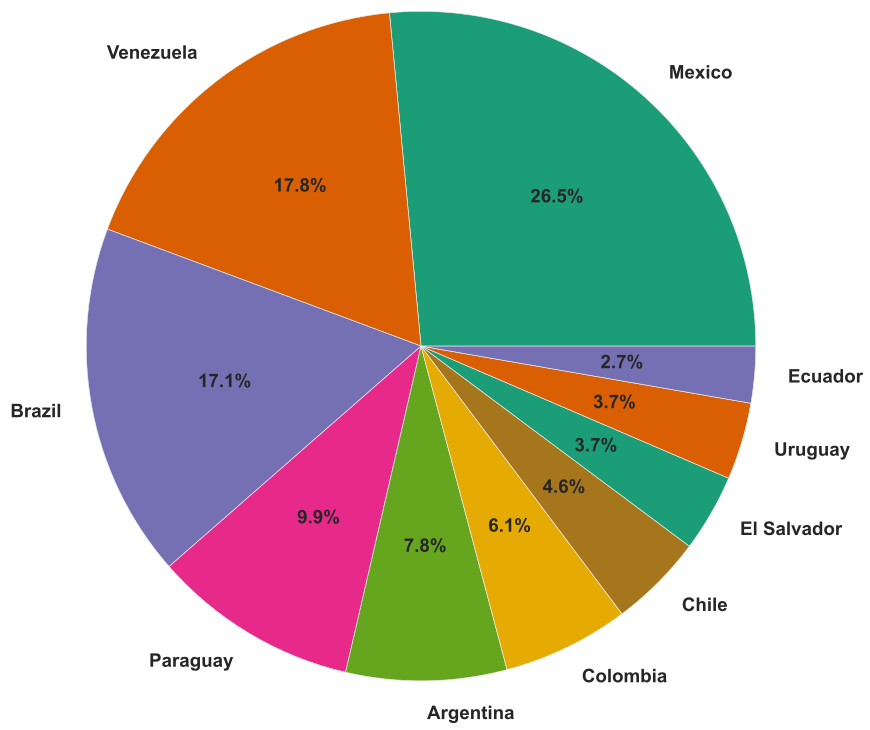
\includegraphics[width=\linewidth]{gsr_distribution}
  \caption{GSR distribution from 2012-11 to 2014-03.}
  \label{fig:gsrdistribution}
\end{subfigure}%
\begin{subfigure}{\columnwidth}
  \centering
  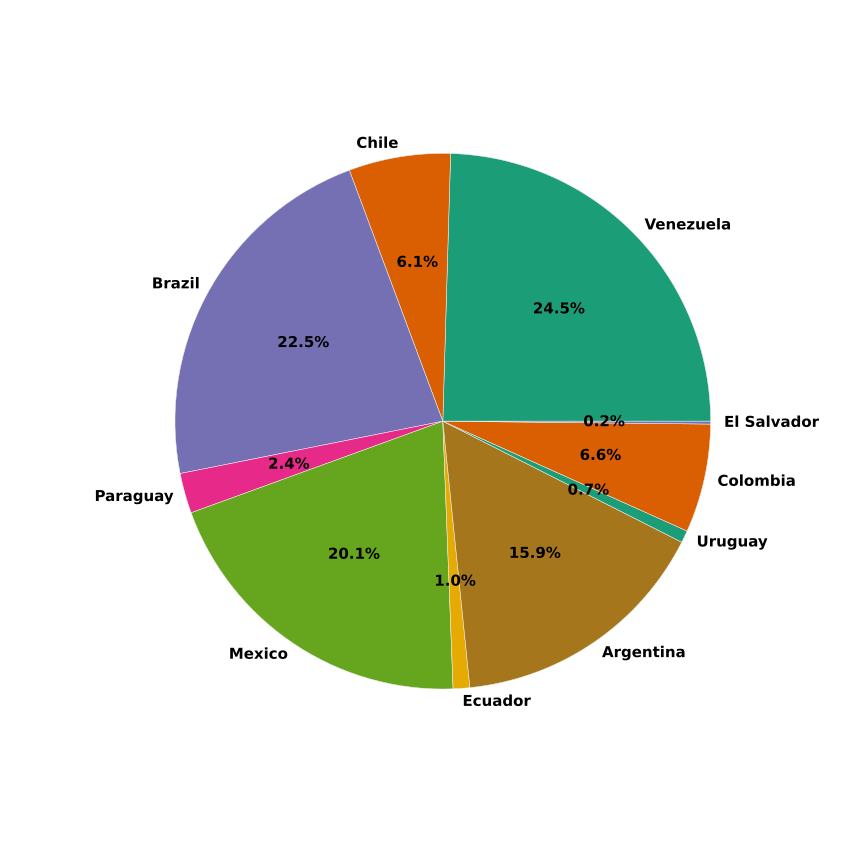
\includegraphics[width=\linewidth]{pp_dist}
  \caption{Alerts distribution from 2012-11 to 2014-03.}
  \label{fig:ppdistribution}
\end{subfigure}
\caption{Distribution of alerts and GSR events across the countries studied in this paper.}
\label{fig:distribution}
\end{figure*}

\noindent
{\bf How does the distribution of protests detected by the system compare with the
actual distribution of protests in the GSR?}
Fig.~\ref{fig:distribution} reveals pie charts of both distributions. As shown, Mexico, Brazil, and Venezuela
experience the lion's share of protests in our region of interest, and the protests detected also match these modes
although not the specific percentages. The smaller countries like Ecuador, El Salvador, and Uruguay do experience
protests but which are not as prominently detected as those for other countries; we attribute this to their smaller
social media footprint (relative to countries like Brazil and Venezuela).\\
\begin{table*}[tb!]
    \small
    \centering
    \caption{\label{tb:sourcewisecomparison} Country-wise breakdown of forecasting performance for different data sources.
QS=Quality Score; Pr=Precision; Rec=Recall; LT=Lead Time.
AR=Argentina; BR=Brazil; CL=Chile; CO=Colombia; EC=Ecuador;SV=El Salvador; MX=Mexico; PY=Paraguay; UY=Uruguay; VE=Venezuela. A $-$ indicates that the source did not produce any warnings for that country in the studied period.}
\vspace{-2mm}
    \begin{tabular}{|*{17}{c|}}
        \hline
        & \multicolumn{4}{ |c| }{News/Blogs} & \multicolumn{4}{ |c| }{Twitter} & \multicolumn{4}{ |c| }{Facebook} & \multicolumn{4}{ |c| }{Combined}\\
        \hline
         & QS & Pr. & Rec. &LT & QS & Pr. & Rec. & LT & QS & Pr. & Rec. & LT & QS & Pr. & Rec. & LT\\
        \hline
        AR &3.14&0.32&0.69&3.94&3.52&{\bf0.78}&0.14&3.14&{\bf3.70}&0.50&0.04&3.00&3.02&0.36&{\bf0.80}&{\bf4.50}\\
        BR &3.14&0.48&0.54&{\bf5.85}&-&-&-&-&{\bf3.62}&{\bf0.76}&0.18&2.46&3.28&0.49&{\bf0.65}&5.15\\
        CL &3.06&0.91&0.67&5.40&{\bf3.52}&{\bf1.00}&0.23&4.29&-&-&-&-&3.16&0.83&{\bf0.80}&{\bf5.92}\\
        CO &2.74&0.90&0.56&{\bf7.44}&3.30&{\bf1.00}&0.15&2.43&{\bf4.00}&{\bf1.00}&0.02&2.00&2.88&0.84&{\bf0.65}&6.47\\
        EC &-&-&-&-&{\bf2.32}&{\bf1.00}&{\bf0.06}&{\bf17.00}&-&-&-&-&{\bf2.32}&{\bf0.50}&{\bf0.06}&{\bf17.00}\\
        MX &2.96&0.88&0.25&{\bf3.69}&3.14&{\bf1.00}&0.02&1.43&{\bf3.72}&0.67&0.01&2.00&3.00&0.87&{\bf0.27}&3.51\\
        SV &{\bf3.22}&{\bf1.00}&{\bf0.03}&{\bf1.0}&-&-&-&-&-&-&-&-&{\bf3.22}&{\bf1.0}&{\bf0.03}&{\bf1.0}\\
        PY &3.38&{\bf1.00}&{\bf0.16}&9.11&3.84&{\bf1.00}&0.04&{\bf11.40}&3.96&{\bf1.00}&0.01&2.00&3.60&0.96&{\bf0.20}&9.35\\
        UY &{\bf3.24}&{\bf1.00}&{\bf0.29}&{\bf2.40}&-&-&-&-&-&-&-&-&3.24&{\bf1.00}&{\bf0.29}&3.24\\
        VE &{\bf3.80}&{\bf1.00}&0.36&{\bf3.27}&3.68&0.97&0.33&2.39&-&-&-&-&3.64&0.99&{\bf0.69}&2.88\\
        ALL &3.34&0.69&0.35&{\bf4.57}&3.62&{\bf0.97}&0.15&2.82&3.66&0.74&0.03&2.44&3.36&0.73&{\bf0.51}&4.08\\
        \hline
    \end{tabular}
\end{table*}

\noindent
{\bf Are there country-specific selective superiorities for the different data sources considered here?}
Table~\ref{tb:sourcewisecomparison} presents a breakdown of perfomance, country-wise and source-wise, of 
of our approach for a recent month, viz. March 2014.
It is clear that the multiple data sources are necessary to achieve a high recall and that by and large
these sources are providing mutually exclusive alerts. (Note also that some data sources do not produce alerts for specific
countries.) Between Twitter and Facebook, the former is a better
source of alerts for countries like Chile and the latter is a better source for Argentina, Brazil, Colombia, and Mexico.
News and blogs achieve higher recall than social media sources indicating that most plans for protests are announced
in established media. They are also
higher quality sources for alerts in countries like El Salvador, Paraguay, and Uruguay.
Finally, note that news and blogs offer a much higher lead time (4.57 days) 
as compared to that for Facebook (2.44 days) or for Twitter (2.82 days). The quality scores are
further broken down in Table~\ref{tb:modelwisecomparison} into their date and location components.
A longitudunal perspective on quality scores is
given in Fig.~\ref{fig:monthlyqs}. Note that in general Twitter tends to have a higher quality score
as multiple re-tweets of future event mentions is a direct indicator of the popularity of an event as 
well as the intent of people to join an event. 
In contrast, mentions of future events in news do not directly shed any insight into popularity or people's
support for the event's causes.\\

\begin{table*} %[tb!]
\centering
\caption{Comparing the location and date scores of different sources in specific countries.
AR=Argentina; BR=Brazil; CL=Chile; CO=Colombia; EC=Ecuador;SV=El Salvador; MX=Mexico; PY=Paraguay; UY=Uruguay; VE=Venezuela. A $-$ indicates that the source did not produce any warnings for that country in the studied period.}
\vspace{-2mm}
\label{tb:modelwisecomparison}
%\vspace{-1em}
\begin{tabular}{||l|*{17}{c|}}
\hline
Source& & AR & BR & CL & CO & EC & SV & MX & PY & UY & VE & All\\
\hline
\multirow{2}{*}{News/Blogs} &LS &0.82&0.76&0.75&0.60&-&{\bf0.75}&0.66&0.79&{\bf0.79}&{\bf0.95}&0.81\\
                            &DS&0.75&0.81&0.78&0.77&-&{\bf0.86}&0.82&0.90&{\bf0.83}&{\bf0.95}&0.86\\
\hline
\multirow{2}{*}{Facebook} &LS &{\bf1.0}&{\bf0.92}&-&{\bf1.00}&-&-&{\bf0.86}&{\bf0.98}&-&-&{\bf0.93}\\
                          &DS&0.85&{\bf0.89}&-&{\bf1.00}&-&-&{\bf1.00}&{\bf1.00}&-&-&0.90\\
\hline
\multirow{2}{*}{Twitter} &LS &0.88&-&{\bf0.84}&0.81&{\bf0.45}&-&0.71&{\bf0.98}&-&0.91&0.89\\
                         &DS&{\bf0.88}&-&{\bf0.92}&0.84&{\bf0.71}&-&0.86&0.94&-&0.93&{\bf0.92}\\
\hline
\end{tabular}
\vspace{-4mm}
\end{table*}

\noindent
{\bf How did our system fare in detecting key country-wide protests?}
The recent Venezuelan protests against President Nicolas Maduro and the Brazilian Protests during June 2013 against bus fare hike were two significant protests during our period of evaluation. Fig.~\ref{fig:venezuela_feb} and
Fig.~\ref{fig:brazil_june} describe our performance under these two situations illustrating the count
of protests detected against the GSR. Notice that our system was able to 
identify the Venezuelan protests much better than the Brazilian protests. This is because there was a significant amount
of spontaineity to the Brazilian protests; they arose as discontent about bus fare increases but later morphed into a broader
set of protests against government and most of these subsequent protests were not planned.\\

\noindent
{\bf What is the tradeoff between lead time and quality?}
Fig.~\ref{fig:leadTimeVsQS} shows that the QS of the planned protest model decreases (as expected) with lead time, initially, but
later rises again. The higher quality scores toward the right of Fig.~\ref{fig:leadTimeVsQS} are primarily due to
Facebook event pages.\\

\noindent
{\bf How does the method perform under stringent matching criteria?}
Fig.~\ref{fig:matchinginterval} shows the perfomance of the model when the matching window is varied from 7 to 1 in steps. 
We can see that the performance degrades quite gracefully even under the strict matching interval of a 1-day difference.\\

\noindent
{\bf What is the distribution of quality scores?}
The clear mode toward the right side of the Fig.~\ref{fig:doubleHump} signifies that a majority of the planned 
protest alerts are of high quality. Further, the quality score distribution is unimodal suggesting that the careful
reasoning of locations and date normalization are crucial to achieving high quality.

\begin{figure*}
\centering
\begin{subfigure}{\columnwidth}
  \centering
  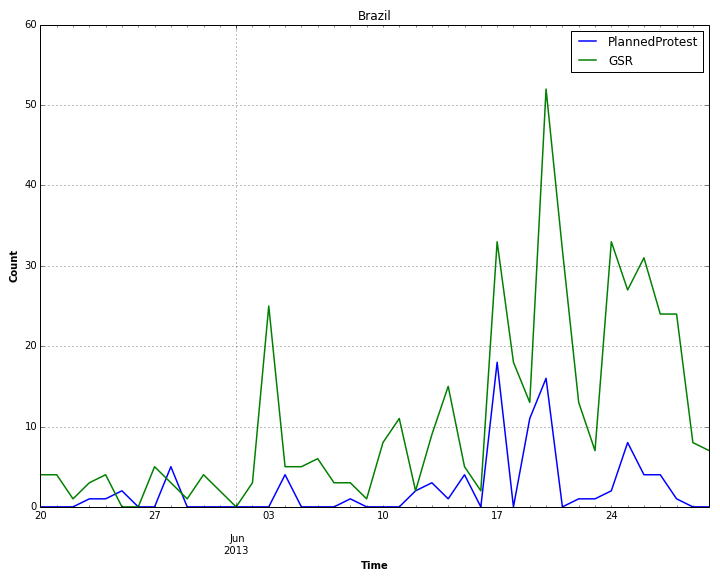
\includegraphics[width=\linewidth]{brazil_june}
  \caption{System Performance during Brazilian Spring}
  \label{fig:brazil_june}
\end{subfigure}%
\begin{subfigure}{\columnwidth}
  \centering
  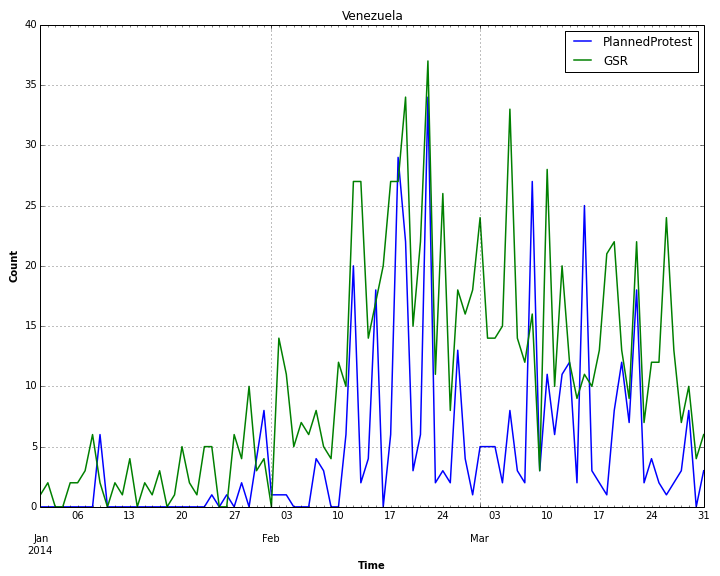
\includegraphics[width=\linewidth]{venezuela}
  \caption{Venezuelan Protests}
  \label{fig:venezuela_feb}
\end{subfigure}
%\begin{subfigure}{\columnwidth}
%  \centering
%  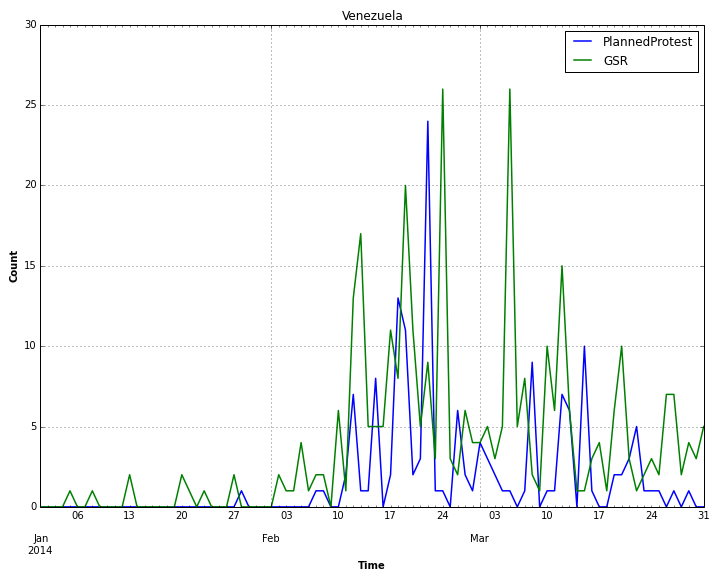
\includegraphics[width=\linewidth]{venezuela_violent}
%  \caption{Venezuelan Violent Protests}
%  \label{fig:venezuela_violent}
%\end{subfigure}%
\begin{subfigure}{\columnwidth}
  \centering
  
\includegraphics[width=\linewidth]{monthlyqs}
  \caption{Quality Score over the months}
  \label{fig:monthlyqs}
\end{subfigure}
\begin{subfigure}{\columnwidth}
  \centering
  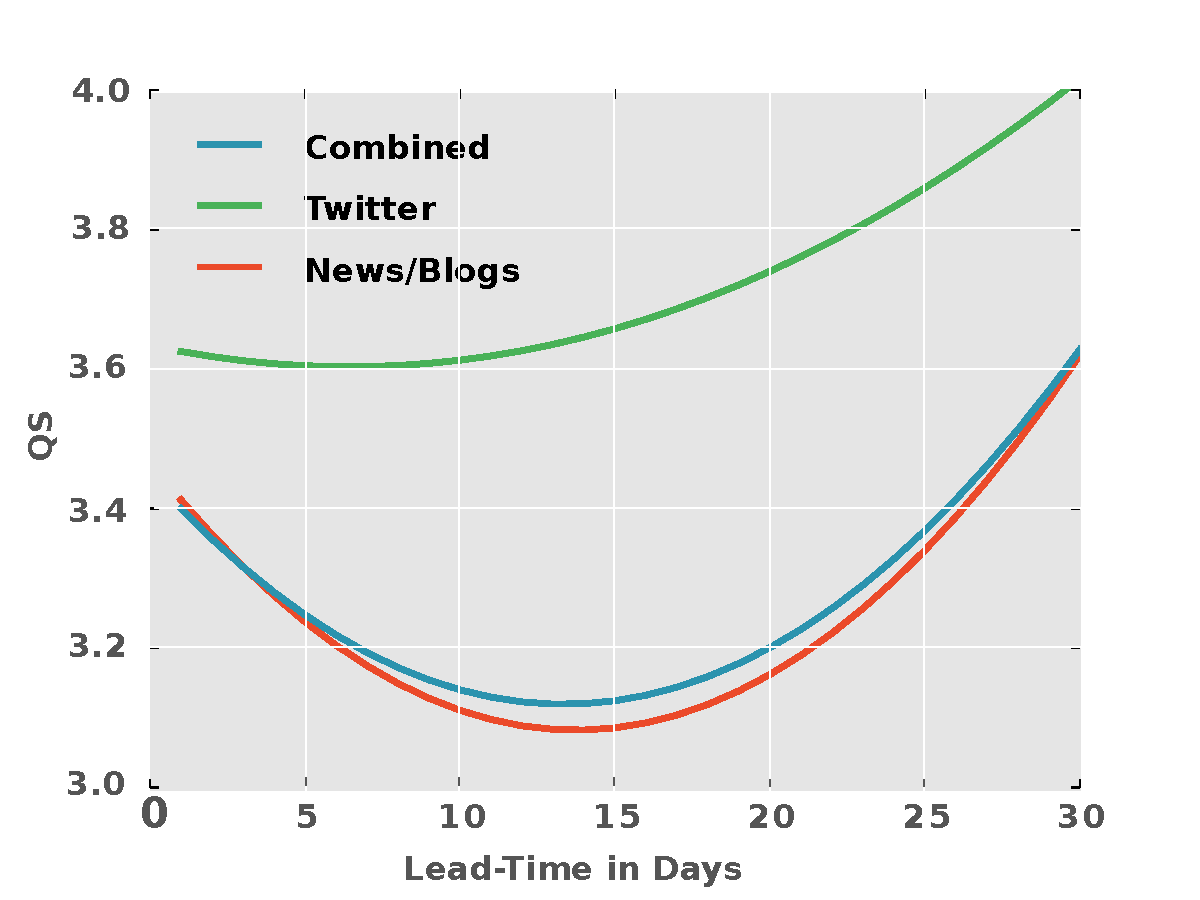
\includegraphics[width=\linewidth]{leadTimeVsQS}
  \caption{Lead-Time vs Quality Score}
  \label{fig:leadTimeVsQS}
\end{subfigure}%
\begin{subfigure}{\columnwidth}
  \centering
  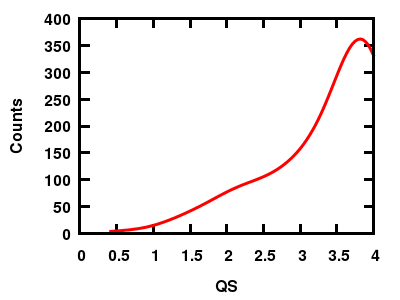
\includegraphics[width=\linewidth]{doubleHump}
  \caption{Quality Score Distribution}
  \label{fig:doubleHump}
\end{subfigure}
\begin{subfigure}{\columnwidth}
  \centering
  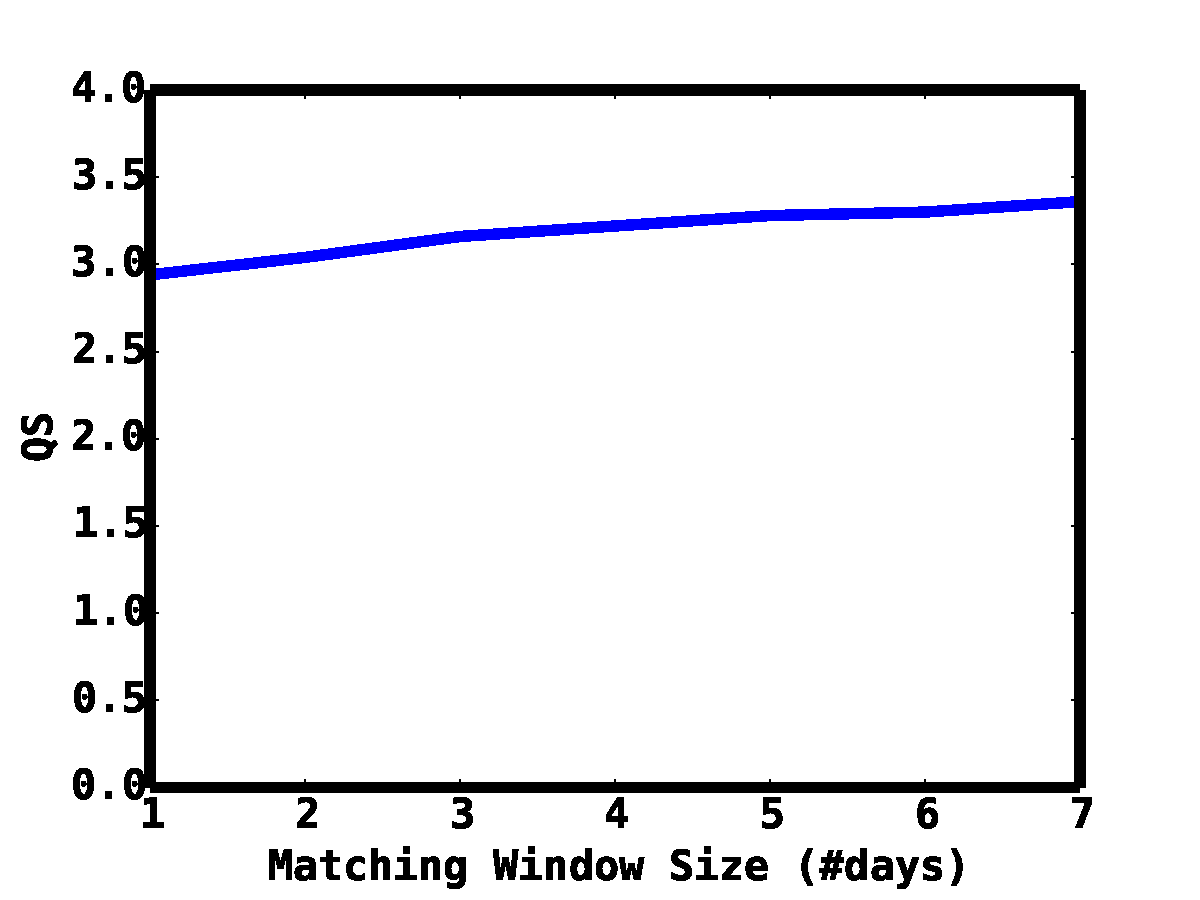
\includegraphics[width=\linewidth]{matchingwindow}
  \caption{QS vs Matching Interval Trade-Off}
  \label{fig:matchinginterval}
\end{subfigure}%
\caption{Experiments}
\end{figure*}

%\begin{figure}
%    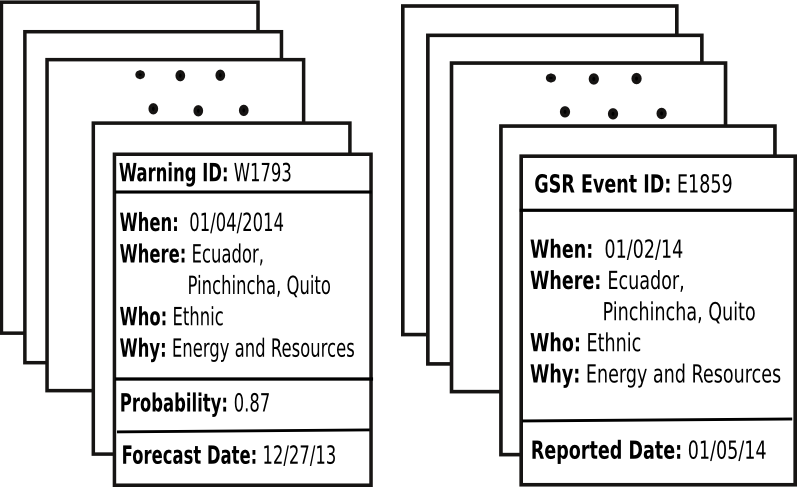
\includegraphics[width=0.5\textwidth]{alertstructure}
%    \caption{Structure of an Alert}
%    \label{fig:alertstructure}
%\end{figure}
%\begin{figure}
%    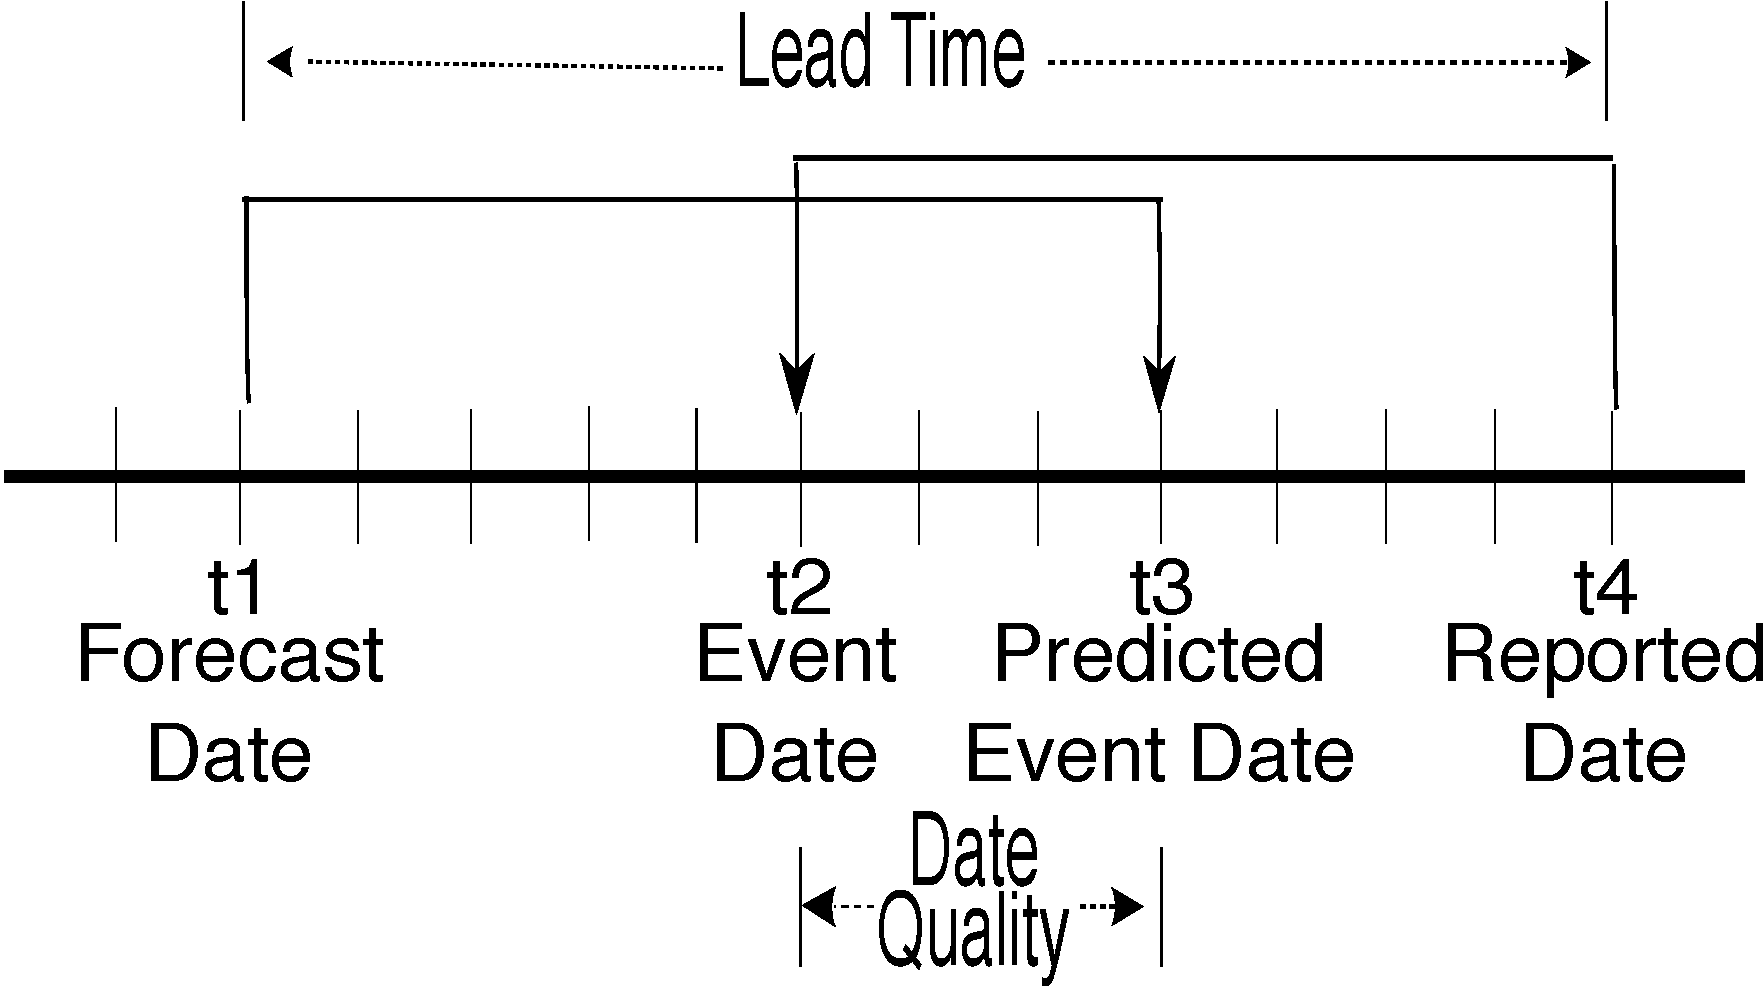
\includegraphics[width=0.5\textwidth]{timeline}
%    \caption{Matching Timeline}
%    \label{fig:timeline}
%\end{figure}
